\documentclass[twoside]{protokoll}
\usepackage{graphicx}
\usepackage{tabularx} % for better table formatting
\usepackage{booktabs} % for better table formatting
\usepackage{float} 
\praktikum{I}
\usepackage{subfig}
\usepackage{amsmath}

\versuchsgebiet{(E-Lehre)}


\teilnehmer{Maximilian Carlos Menke, 434170}
\teilnehmer{Andrea Roth, 428396}
\gruppe{A3}

\begin{document}
 
\section{1E3 Gekoppelte LC-Schwingkreise}

\begin{aufgabe}{Grundlagen}
  Knappe Beschreibung der theoretischen Grundlagen, Angabe der
  benötigten Formel(n), ohne Herleitung. Definition der verwendeten
  Formelzeichen.
\end{aufgabe}

\begin{aufgabe}{Versuchsaufbau und Versuchsdurchführung}
  Beschreibung des Versuchsaufbaus einschließlich
  Schaltbild. Beschreibung der Versuchsdurchführung: verwendete
  Messwerterfassungseinstellungen, Messbereiche, Triggerbedingungen,
  etc.
\end{aufgabe}

\subsection{Kurze Zusammenfassung des Aufbaus und Durchführung}

Detailierter Aufbau und Durchführung zu den einzelnen Versuchsteilen, finden Sie am Anfang von den jewailigen Abschnitten. 
Hier soll der Gesamtversuch kurz Dargestellt werden.\\

Der Versuch besteht aus insgesamt 3 Teilen. Für den ersten Teilversuch haben wir zwei LC-Schwingkreise Aufgebaut mit gleichen Bauteilen und die Schwingung in diesen einzelnd gemessen. 
Diese sind Schwingkreise mit jeh einem Kondensator und einer Spule.
Als Wiederstand in der Schalltung liegt nur der Innenwiederstand von Spule und Kondensator und den Kabeln vor. 
An den Schwingkreis wird eine Spannungsquelle angeschlossen, welche mithilfe eines Tasters kurzgeschlossen werden kann und den Schwingkreis schließt. 
Der Spannungsverlauf wird über dem Kondensator parallel gemessen. 
Dieser Teilversuch dient dazu den Einzelschwingkreis zu charakterisieren, dies wird Später benötigt zur Auswertung der gekoppelten Schwingkreise.\\

Zur Kopplung der Schwingkreise werden die Spulen nebeneinander gestellt und auch die Spannung am zweiten Kondensator gemessen. Durch drücken des Tasters wird eine Messung gestartet.
Als Einflussfaktoren auf den Kopplungsgrad wird das Variieren des Abstands der Spulen untersucht und der Einfluss eines Eisenkerns\\

Im letzten Teilversuch werden nun beide Kondensatoren mit der gleichen Spannungsquelle geladen. 
So, dass der Strom ein mal gleichsinnig durch die Spulen läuft und ein mal gegensinnig. Die Schwingungen haben wir wieder an beiden Kondensatoren gemessen, und daraus die Frequenzen $f_+$ und $f_-$ bestimmt. 
 

\begin{aufgabe}{Vorversuch: Charakterisierung der verwendeten Bauteile}
  Charakterisieren Sie die verwendeten Bauteile mit Digitalvoltmeter
  bzw. Messbrücke.
\end{aufgabe}

Vor der Durchführung der Versuche, und zum späteren Vergleich der Messungen mit unseren Erwartungen haben wir die Bauteile charakterisiert. Dies haben wir mit einer Messbrücke getan. 

\begin{figure}[H]
    \centering
    \includegraphics[width=0.8\textwidth]{bilder/Messbrücke_10Ohm.pdf}
    \caption{Charakterisierung des 10 $\mu F$ Kondensator}
\end{figure}

In dem Bild zu sehen ist die Messbrücke, an die Stelle wo der Kondensator ist, wir das Bauteil angeschlossen. Das Bild ist noch mit unserem ersten Kondensator, diesen haben wir im Verlauf des Experiments gegen einen kleineren ausgetauscht, und alle Messungen mit dem kleineren wiederholt.\\

Für die Messung haben wir unseren Frequenzbereich von 1kHz eingestellt.
 (In dem Bild auf 100Hz weil wir da noch den 10 $\mu F$ messen, und wir mit diesem geringere frequenzen hatten.) 
So konnten wie sämtliche Bauteile Charakterisieren und sind für unseren zweiten Aufbau (mit kleinerem Kondensator) zu folgenden Ergebnissen gekommen:\\
    
\begin{table}[h]
        \centering
        \begin{tabularx}{0.8\textwidth}{X X c} % adjust width as needed
            \toprule
            \textbf{Bauteil} & \textbf{Messung} & \textbf{Fehler} \\
            \midrule
            Spule 1 & L = 9.023mH &  \\
            & R = 2.344 $\Omega$ & \\
            Spule 2 & L = 8.981mH &  \\
            & R = 2.423 $\Omega$ \\
            Kondensator 1 & 2.301 $\mu$F &  \\
            Kondensator 2 & 2.262 $\mu$F &  \\
            \bottomrule
        \end{tabularx}
        \caption{Ergebnisse der Messung mit dem Multimeter}
        \label{tab:mytable}
    \end{table}

\begin{aufgabe}{Ungekoppelte Schwingung}
  Zeigen Sie den Verlauf der Kondensatorspannungen für den
  ungekoppelten Fall und bestimmen Sie die Schwingungsfrequenz samt
  Messunsicherheit. Vergleichen Sie sie mit Ihrer Erwartung.
\end{aufgabe}

\subsection{Ungekoppelter Schwingkreis}

\subsubsection{Materialien}


Vor Beginn des Versuchs haben wir unsere Bauteile gewählt. Wir hatten uns erst für einen $10\mu F$ Kondensator entschieden und eie Spule mit 500 Windungen.
Dies erachteten wir als Sinnvoll da wir wissen, dass $ f \propto \frac{1}{LC}$ gilt. 

So haben wir eine niedrigere Frequenz als bei kleineren Kondensatoren. 
Diese Spule haben wir gewählt, da eine Spule mit weniger Windungen zwar geringeren Wiederstand hat aber auch eine geringere Kopplung. Eine Spule mit mehr Windungen würde zwar die Kopplung vergrößern, jedoch auch den Wiederstand. \\

Bei den gekoppelten Schwingkreisen, stellten wir jedoch fest, dass bereits ab einem Abstand von 1cm keine Kopplung mehr vorlag. 
Aufgrund dessen haben wir dann unseren $10\mu F$ Kondensator duch einen $2.2 \mu F$ ausgetauscht. \\


Zuerst haben zwei ungekoppelte Schwingkreise aufgebaut mit gleichen Bauteilen.
 
\textbf{Material Liste}
\begin{itemize}
  \item 2x Spule $9mH$
  \item 2x Kondensator $10 \mu F$
  \item Spannungsqelle vom Cassy
  \item Schalter
  \item Kabel
  \item Steckplatte DIN A4
\end{itemize}

\subsubsection{Aufbau}
Der erste Schwingkreis wurde dabei wie unten skizziert aufgebaut.
\begin{figure}[H]
    \centering
    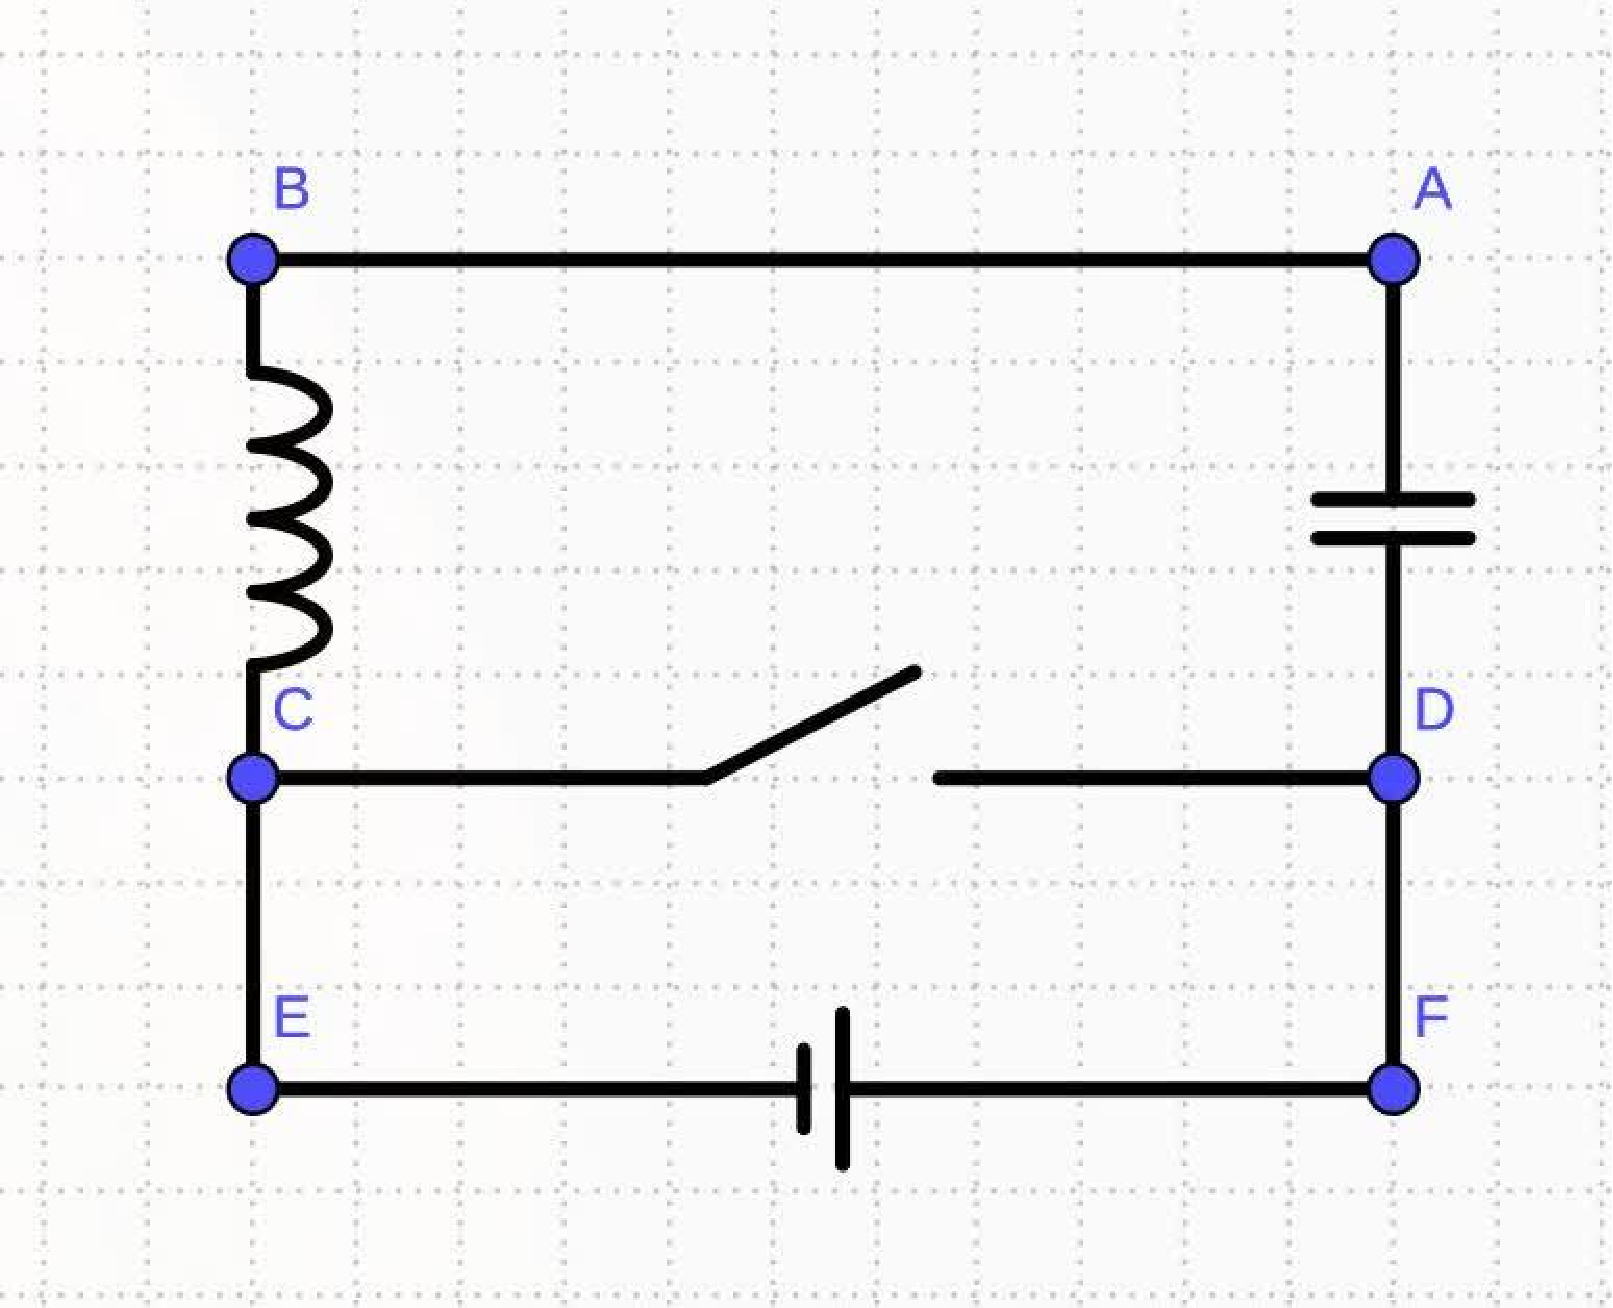
\includegraphics[width=0.8\textwidth]{schaltplan-einzelschwingkreis.pdf}
    \caption{Aufbau der Schwingkreise}
\end{figure}
\begin{figure}[H]
    \centering
    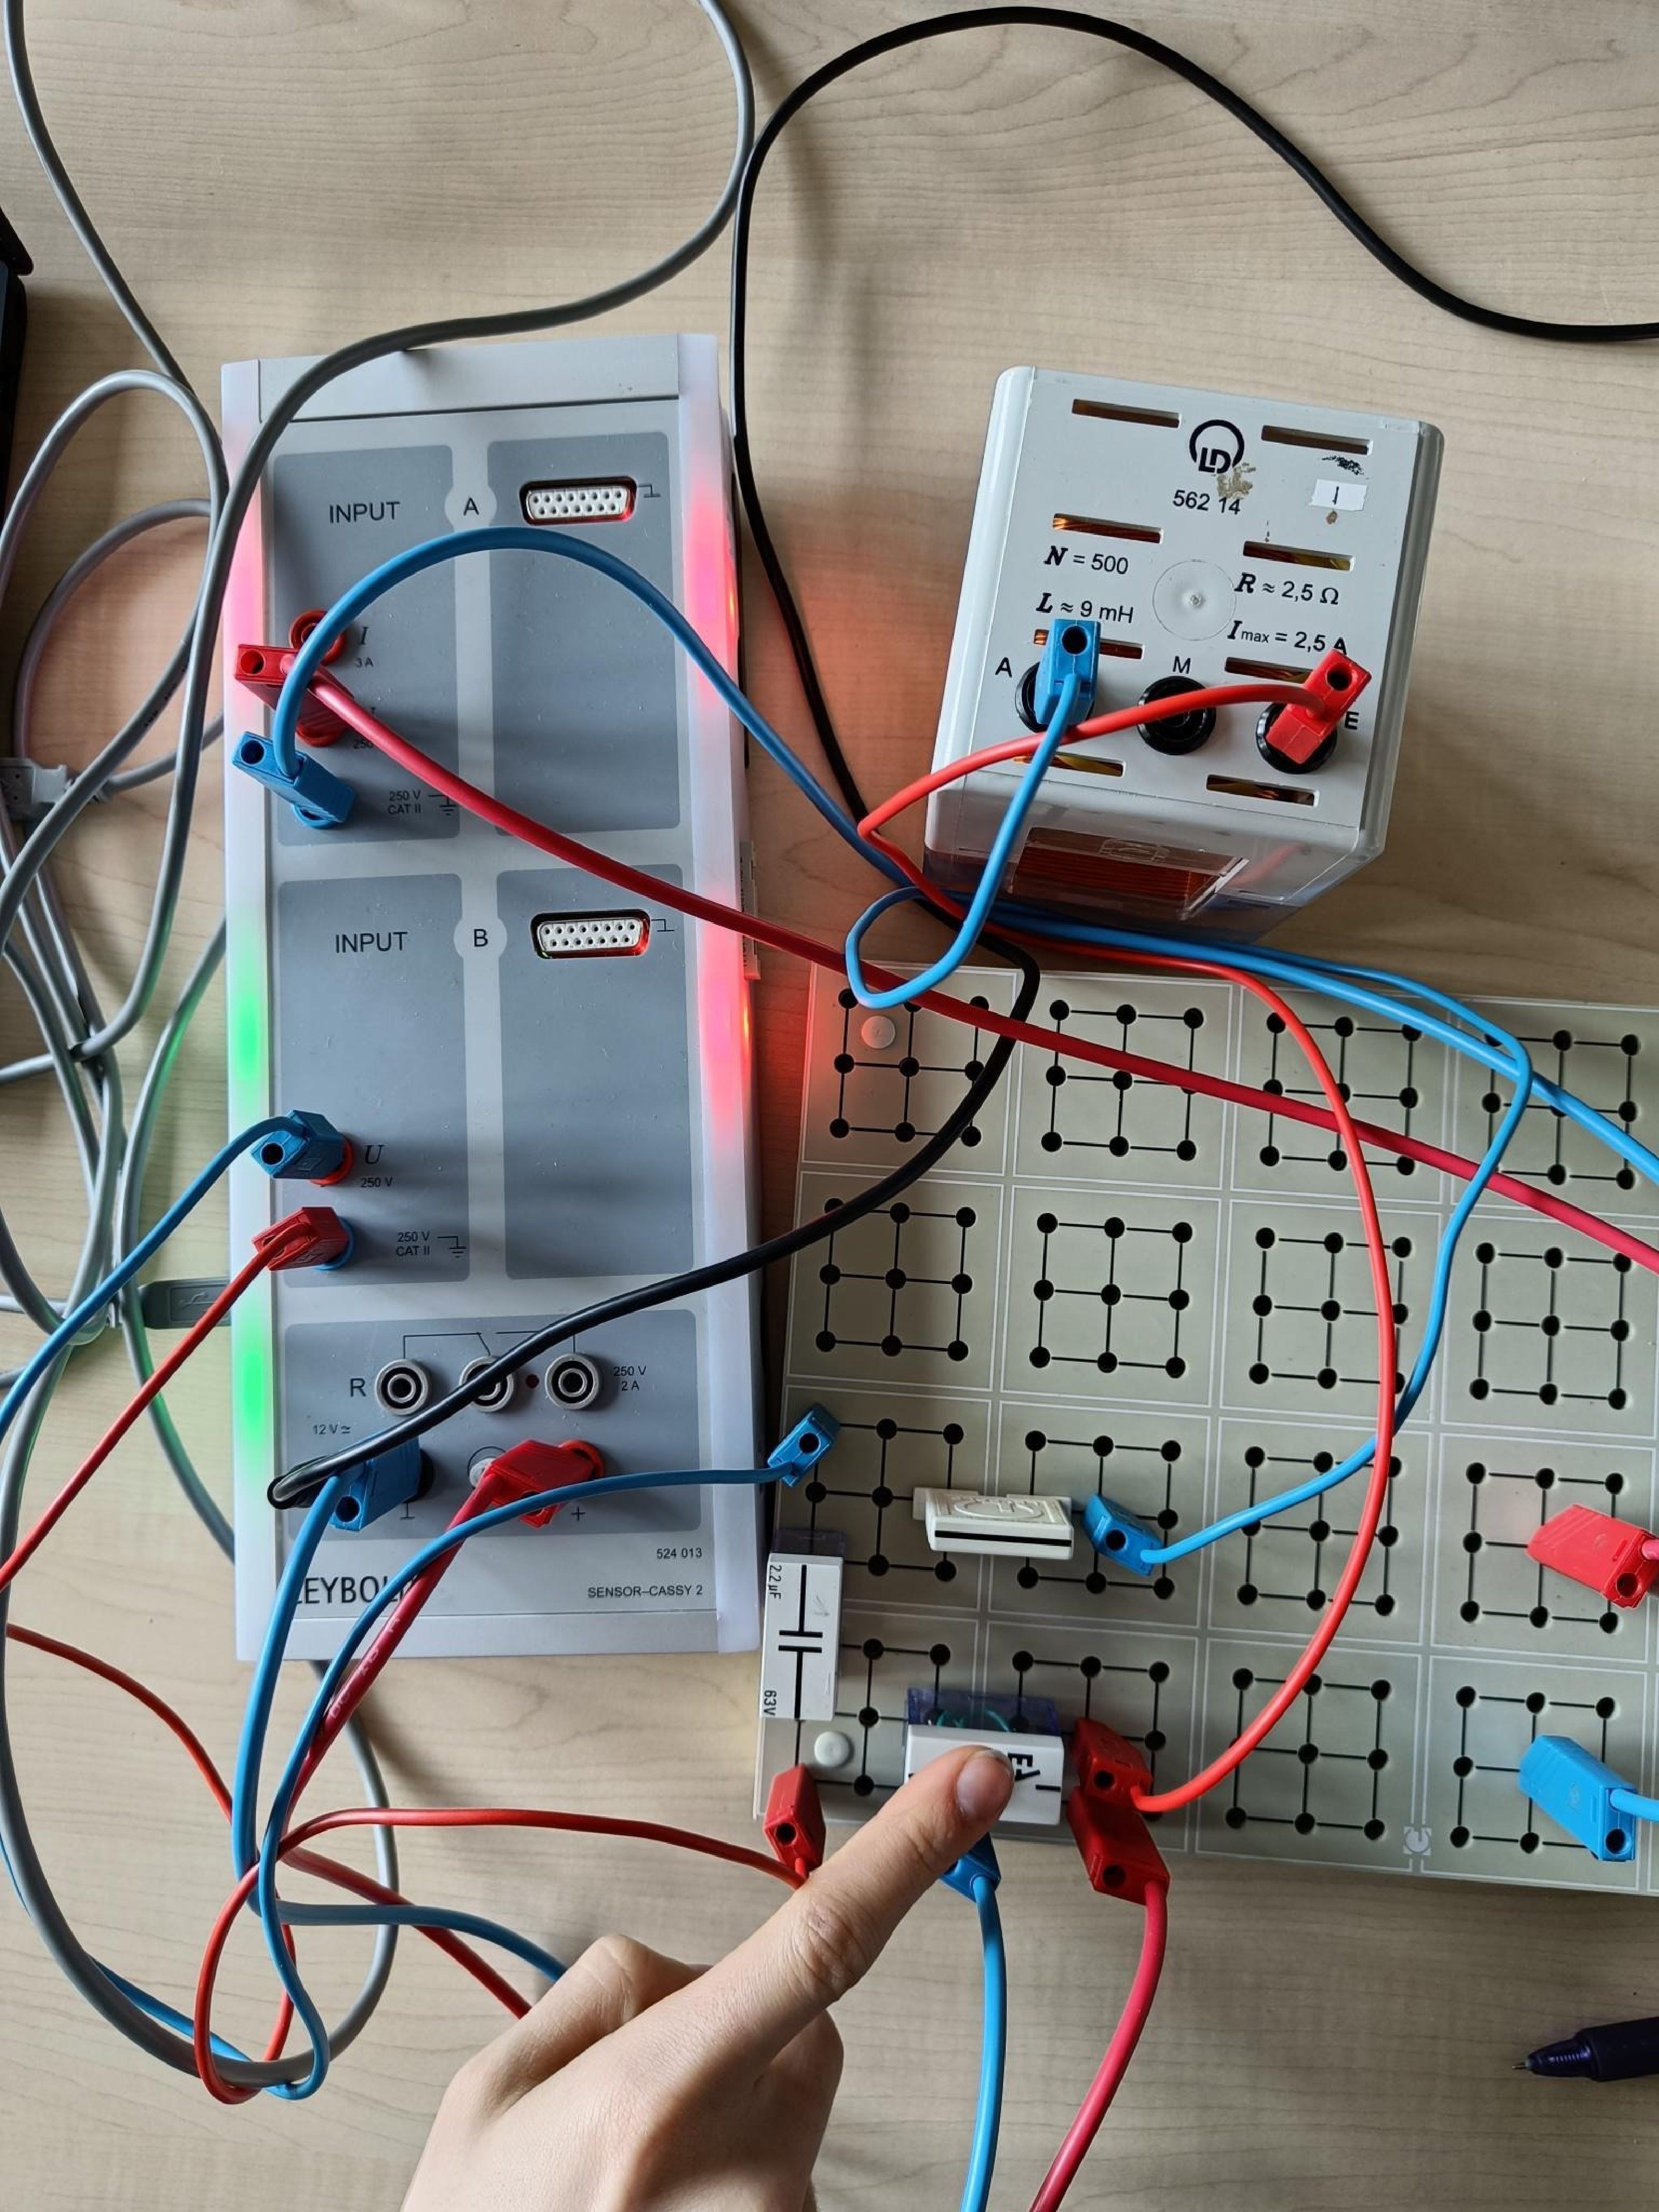
\includegraphics[width=0.4\textwidth]{bilder/schwingkreis1.pdf}
    \caption{Aufbau des 1. Schwingkreises}
\end{figure}
   
Zudem haben wir mit der 2. Spule und dem 2. Kondensator einen zweiten Schwingkreis aufgebaut.
Die Schaltskizze des 2. Schwingkreises ist gleich zu dem des 1.
Insgesammt hatten wir 2 getrennte Schwingkreise, aber nur einen Schalter und eine Spannungsqelle (da wir die Schingkreise später koppeln werden).
Des haben wir die Spannungsqelle und den Schalter dann jeweils umgesteckt, da wir den Kondensator und die Spule einzeln vermessen wollten.




\subsection{Durchführung}
Zuerst haben wir eine Spannung von $U_0 = 6.2V$ angelegt da bei dieser Spannung die Maximale Stromstärke der Spule ( $2.5A$ ) nicht überschritten wird.
Anschließend haben wir ein paar Testmessungen gemacht, um die optimalen Messeinstellungen zu finden.
Diese Testmessungen haben wir aber noch mit unserer 'alten' Kapazität gemacht ( $C = 10 \mu F$ ), aber beim verbauen der neuen wiederholt.
Beim einbauen der neuen haben wir die Messparameter aber wie unten beschieben angepasst.
Dafür haben wir die Periodendauer als Näherung ohne Wiederstand (da dieser für eine grobe Abschätzung vernachlässigbar klein ist) überschlgen:
\begin{equation}
    T = 2 \pi \sqrt{LC} = 2 \pi \sqrt{9mH \cdot 2.2 \mu F} = 884 \mu s
\end{equation}
Nach dem Nequisst Theorem muss die Abtastrate mindestens doppelt so groß sein wie die Frequenz.
Um noch etwas sicherheitspuffer zu haben, und da diese Messung nur eine abschätzung war, haben wir $ 50 \mu s $ als Messintervall gewählt, da dieses mehr als das 10x ist.

Die Länge der Messung beeinflusst dabei die Auflösung der Fouriertransformation (FFT).
 
 
Dabei startet die Schwingung im Schwingkreis in dem Moment, wo man den Taster drückt, da sich jetzt der Kondensator anfangen kann zu entladen.
Damit der Schwingkreis sauber schwingen kann, muss der Taster auch während der gesamten Messung gedrückt bleiben.
Entsprechend haben wir den Trigger vom Cassy auf 6.1V fallende Flanke gestellt um die Messung zu starten.
Dabei haben wir 6.1V gewählt, da so noch der großteil der ersten Schwingungsperiode mit aufgezeichnet wird.
0.1V Abstand (6.2V - 6.1V )war mehr als ausreichend, um nicht spontan gestartet zu werden, aber noch weit genug entfernt um eventuelle Störeffekte vom Schalter kurz nach dem Schalten zu unterbinden.
Den 2. Schwingkreis haben wir dabei 10 mal vermessen, um die Statistische Unsicherheit auf die Frequenz zu bestimmen.
Beim Cassy 



Den 1. Schwingkreis haben wir dabei nur einmal vermessen, da wir davon ausgehen können, das die Statistische Unsicherheit bei beiden Schwingkreisen gleich ist, da wir den gleichen Aufbau verwendet haben und auch sonst gleiche Messbedingungen hatten.

\subsubsection{Rohdaten}

Insgesamt hatten wir also die Kondensatorspannung beim Schwingungsvorgang in zweiten Schwingkreis 10x gemsessen. Und im ersten Schwingkreis ein mal. 
So wie eine Rauschmessung bei 0V und bei ca. 6V. 


\begin{aufgabe}{Gekoppelte Schwingung: Schwebung}
  Stellen Sie für einen festen Kopplungsgrad $k$ eine Schwebung
  dar. Zeigen Sie jeweils die Fourierspektren, bestimmen Sie die
  Eigenfrequenzen und daraus den Kopplungsgrad sowie dessen
  Messunsicherheit. Bestimmen Sie die zeitliche Verschiebung
  $\Delta{}t$ zwischen den beiden Einhüllenden der Schwebungen der
  beiden Kondensatoren und vergleichen Sie sie mit Ihrer
  Erwartung. Stellen Sie dar, wie sich das Frequenzspektrum mit dem
  Abstand der Spulen ändert. Untersuchen Sie die Verstärkung der
  Kopplung durch Verwendung eines Eisenkerns in den beiden Spulen.
\end{aufgabe}


\begin{aufgabe}{Gekoppelte Schwingung: gleich- und gegensinnige Anregung}
  Stellen Sie für einen festen Kopplungsgrad $k$ nacheinander die
  beiden Fundamentalschwingungen dar. Zeigen Sie jeweils die
  Fourierspektren und bestimmen Sie die zugängliche
  Eigenfrequenz. Berechnen Sie den Kopplungsgrad sowie dessen
  Messunsicherheit. Vergleichen Sie mit den Werten aus der Schwebung.
\end{aufgabe}
   
   
\end{document}
